\documentclass[conference]{IEEEtran}
\usepackage{graphicx,booktabs,array}
\usepackage[T1]{fontenc}
\usepackage[utf8]{inputenc}
\usepackage{url}
\graphicspath{{figures/}}
\begin{document}
\title{Verify, Diagnose, Adapt: Agent-Validated Prerequisite Graphs for Student-Adaptive Learning Paths}
\author{\IEEEauthorblockN{Shreeya Kiran Khairnar}
\IEEEauthorblockA{Dept. of Computer Science \& Engg. \\ M S Ramaiah Institute of Technology \\ Bengaluru, India \\ shreeyakiran04@gmail.com}
\and
\IEEEauthorblockN{Vaidehi Kumawat}
\IEEEauthorblockA{Dept. of Computer Science \& Engg. \\ M S Ramaiah Institute of Technology \\ Bengaluru, India \\ vaidehikumawat2020@gmail.com}
\and
\IEEEauthorblockN{Sneha Debnath}
\IEEEauthorblockA{Dept. of Computer Science \& Engg. \\ M S Ramaiah Institute of Technology \\ Bengaluru, India \\ snehadebnath2608@gmail.com}
\and
\IEEEauthorblockN{Shrestha Sunil}
\IEEEauthorblockA{Dept. of Computer Science \& Engg. \\ M S Ramaiah Institute of Technology \\ Bengaluru, India \\ shrestha.sunil051@gmail.com}
\and
\IEEEauthorblockN{Sangeetha J}
\IEEEauthorblockA{Dept. of Computer Science \& Engg. \\ M S Ramaiah Institute of Technology \\ Bengaluru, India}}
\maketitle
\noindent\fbox{\parbox{0.95\columnwidth}{\footnotesize\emph{Work-in-progress manuscript. The system is built and its evaluation is running. Results marked ``pending'' have not been obtained yet, and every number shown is preliminary.}}}
\begin{abstract}
Students often struggle with an advanced topic because they missed something it depends on, yet course material rarely says which concepts depend on which, or which gap a particular student has. Large language models (LLMs) can propose prerequisite relations cheaply, but they also propose relations that sound right without being needed. We present a system that goes from raw course files to a personalized learning path. An LLM proposes prerequisite edges, and an independent validation agent checks each one against retrieved course text, a second model and graph-consistency rules, then accepts it, rejects it or sends it for human review. A short adaptive quiz over the validated graph estimates what a student knows, a tracer suggests which concept caused a wrong answer, and the student receives a path with cited sources. We also study a counterfactual ``necessity test'' in which an LLM simulates a learner who lacks a concept. This paper reports the design and preliminary findings. The necessity test was unstable across settings on three example edges, so it does not influence decisions in the current agent. A real-textbook run exposed prompt truncation and an order bias in discovery, which we corrected in the design. On 500 simulated students over a five-concept example graph, adaptive diagnosis used 14.4\% fewer questions than asking every concept at similar accuracy (0.866 vs. 0.870), but only when student knowledge followed the graph. The main evaluation of validation on public benchmarks and full courses is pending.
\end{abstract}
\begin{IEEEkeywords}
prerequisite relation discovery, educational knowledge graph, large language models, LLM validation, adaptive diagnosis, personalized learning paths
\end{IEEEkeywords}
\section{Introduction}
Most of what students learn builds on something they learned earlier. A student who says ``I don't understand AVL trees'' may have no trouble with balancing at all. They may never have understood the ordering rule of binary search trees (BSTs). Telling them to revise AVL trees does not find that gap. The useful answer depends on two things: the dependency structure of the course, and where in that structure this student's knowledge stops.

An instructor could draw a prerequisite map by hand, but that is slow for a course with hundreds of concepts. LLMs can propose such maps at low cost @@CITEpan\_kg@@, but they also generate plausible errors @@CITEji\_halluc@@. In a graph, one wrong edge can add an unnecessary branch to every learning path that passes through it.

We ask two linked questions. Can LLM-proposed prerequisite edges be checked, so that only supported edges enter the course graph? And can one validated course graph give each student a different path, based on what that student already knows?

We do not claim that prerequisite discovery is new. Our contributions are:

\begin{enumerate}
\item \textbf{An independent validation agent} that combines course-text evidence with verified quotes, a semantic judgment from a different model, and graph-consistency rules, with three outcomes: accept, reject or human review.
\item \textbf{A study of a counterfactual necessity test}, in which an LLM simulates a learner who lacks a concept. We report honestly that it was unstable in our runs.
\item \textbf{Graph-guided adaptive diagnosis}, which uses the validated graph to choose the next quiz question and to infer knowledge of related concepts.
\item \textbf{Root-cause tracing}, which reads the option a student chose and ranks which concept in the prerequisite chain most likely caused the error.
\item \textbf{Personalized, explainable paths and impact-ranked human review}: one course graph, a different path per student, with uncertain edges ranked by how many student paths they would change.
\end{enumerate}
The system is implemented end to end, including a website that takes uploaded course files. Section VI separates what has been measured from what is pending.

\section{Related Work}
\subsection{Prerequisite Relation Learning}
Early work used Wikipedia links and crowdsourced judgments \cite{talukdar}. RefD measures asymmetry in links between related pages \cite{refd}. Others learned from MOOC features @@CITEpan\_mooc@@, university course dependencies \cite{liang17} and active learning \cite{liang18}. PREREQ \cite{prereq} and LectureBank \cite{lecturebank} moved toward learned representations. More recently, PCPL applies prompt learning \cite{pcpl}, LCPRE uses learning-path information \cite{lcpre}, and GKROM optimizes relations globally \cite{gkrom}. Most of this work measures pairwise accuracy on curated benchmarks. We treat discovery as an input and focus on what happens after an LLM proposes an edge.

\subsection{Educational Knowledge Graphs and Paths}
ACE combines machine learning with expert input to reduce the effort of building prerequisite graphs \cite{ace}. InstructKG builds graphs from lecture material and reports that LLM extraction without instructor-grounded signals yields inaccurate pedagogical graphs \cite{instructkg}, which matches what we observed. Prerequisite information has also been used to recommend learning objects \cite{chanaa}. Our paths differ per student, and each step keeps its evidence.

\subsection{Student Modeling}
Knowledge Space Theory models feasible knowledge states under a prerequisite relation, so a few questions can place a learner in a state \cite{kst}. Our diagnosis uses the same idea, but the relation is proposed by an LLM and checked automatically instead of being elicited from experts. Knowledge tracing estimates mastery over time from many interactions \cite{bkt}, \cite{dkt}. A new course has no such logs, whereas our approach starts from course material alone.

\subsection{Verification of LLM Outputs}
Common countermeasures include grounding in retrieved text \cite{rag}, sampling and majority voting \cite{selfcons}, and using one model to judge another \cite{judge}. We apply these ideas to a structured output, a graph edge, where some constraints such as acyclicity can be checked exactly. Our baselines include a single judge and a self-consistency judge, so the effect of more LLM calls can be separated from the effect of independent checks.

\section{Problem Formulation}
A course is a set of documents split into chunks, each keeping its source document and page. Extraction gives a set of concepts. A concept A is a \emph{hard} prerequisite of B if B cannot be understood without A, and a \emph{soft} prerequisite if A clearly helps but is not required. The course graph is a directed acyclic graph (DAG) of validated edges, and it is shared by all students. Prerequisite edges belong to the concepts; what differs per student is a knowledge state, a mastery value for each concept. A concept counts as mastered when its mastery is above 0.8. For a target t, the personalized path is the target and its ancestors minus the mastered concepts, in topological order.

\section{Proposed System}
\begin{figure}[!t]
\centering
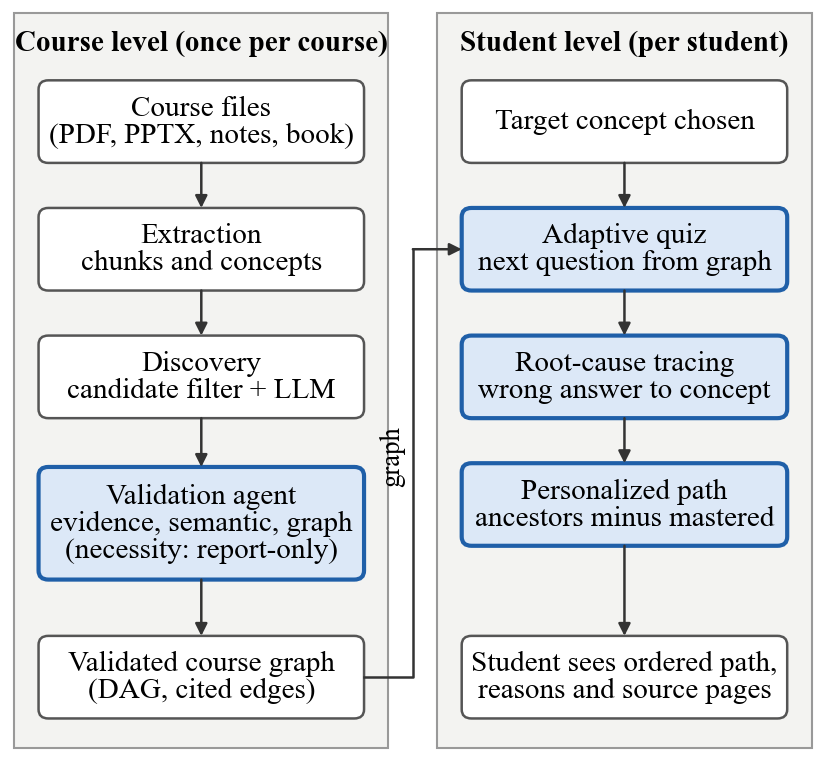
\includegraphics[width=\columnwidth]{pipeline.png}
\caption{System overview. The course level runs once per course and the student level runs per student. Every stage exchanges schema-validated JSON files.}
\end{figure}
\subsection{Extraction}
PDF, PPTX, Markdown, TXT and DOCX files are split into chunks of at most 500 words that keep their source. An LLM lists the concepts in each chunk, and near-duplicate names are merged by embedding similarity (all-MiniLM-L6-v2 \cite{sbert}), with aliases kept. Extraction stops with an error instead of silently falling back if the LLM or the embedding model is unavailable, and the method used is recorded in the output.

\subsection{Dependency Discovery}
Sending every concept pair to an LLM is too expensive, so a pair is kept only if there is a signal: the concepts share a chunk, one is named in the other's definition or source text, or their embeddings are similar. The proposer (qwen2.5:7b-instruct) receives up to four excerpts and answers one neutral question: A before B, B before A, or neither, with a strength and a confidence. Concepts are presented in a fixed order that does not depend on the course (prompt version v3, described in Section VI-B).

\subsection{Validation Agent}
Every proposed edge is treated as a claim. The agent uses a different model (llama3.1:8b) and its own prompts, because a model that finds an edge plausible once will tend to do so again. All calls use a fixed seed and are cached, with the model, prompt version and temperature recorded.

\textbf{Graph check (no LLM).} Each edge is labelled self-loop, duplicate, contradiction (both directions proposed), cycle, redundant (implied by a longer path) or ok.

\textbf{Evidence check.} The agent gathers the chunks discovery cited plus the top three retrieved by embedding similarity. The model grades whether the excerpts support learning A before B as strong, medium, weak or none, and it must quote the text. A quote is kept only if it appears verbatim in the cited chunk, and a strong or medium grade with no verifiable quote is capped at weak. Every displayed quote is therefore traceable to a document and page.

\textbf{Semantic check.} The model grades the edge from concept names and descriptions only, so it does not share the evidence check's input. Used alone, it is also our single-judge baseline.

\textbf{Necessity test.} A question writer creates questions on B without naming A. A simulated learner answers them with A forbidden. A control run uses the same prompt with an unrelated concept C forbidden instead, which absorbs the penalty of being told ``you never learned X''. A separate grader, blind to the run, scores both. The necessity gap is the control score minus the without-A score. Answers that still use A's name are counted as leakage. Because of the instability reported in Section VI-D, this test is \emph{report-only} in the current agent: it has weight 0 and never changes a decision.

\textbf{Decision rule.} Self-loops and duplicates are rejected, and redundant edges are rejected with the reason ``implied by \ldots{}''. Contradictory or bidirectional edges go to human review, and a cycle is never accepted. Otherwise grades map to points (1, 0.67, 0.33, 0), and the score is the mean over active checks. An edge is accepted if the score is at least 0.6 and no active check says none. It is rejected if the score is below 0.35, or if evidence and semantic are both weak or none. Otherwise it goes to review. These values are a first choice, not yet calibrated.

\subsection{Impact-Ranked Human Review}
For each edge sent to review, we compare every simulated student's path with and without the edge. Its impact is the share of paths that change, and the queue is sorted by impact. Edges that would close a cycle are flagged as blocking and come first. On the website, a teacher accepts or rejects an edge, and an edge that would close a cycle is never added.

\subsection{Adaptive Diagnosis and Personalized Path}
Each concept starts at mastery 0.5. The next question targets a concept near the middle of the uncertain part of the target's prerequisite chain (mastery between 0.2 and 0.8). A correct answer sets that concept to 0.9 and its ancestors to at least 0.85. A wrong answer sets it to 0.1 and keeps its prerequisites in question. The latest direct answer on a concept always overrides inference. Quiz items are generated by an LLM from the course chunks, and an item is dropped if its answer is not among its options.

\subsection{Root-Cause Tracing}
Given a wrong answer on concept T, the candidates are T and its ancestors over accepted edges. An LLM reads the question, the options, the chosen option and this chain, and ranks the candidates with a one-line explanation. Output is restricted to the chain. Two baselines also rank the chain: \emph{blame the target}, and \emph{blame the nearest prerequisite} (lowest mastery, then hard before soft, then concept ID).

\section{Experimental Setup}
\subsection{Datasets}
\textbf{Our courses} use openly licensed material so the work can be reproduced (Table I): \emph{ds101} uses \emph{Open Data Structures} \cite{ods} and OpenDSA modules \cite{opendsa} for AVL trees, general trees and recursion, and \emph{ml101} uses \emph{Dive into Deep Learning} \cite{d2l} and \emph{Introduction to Modern Statistics} \cite{ims} for logistic regression.

\begin{table}[!t]
\caption{Our Course Corpora}
\centering\footnotesize
\begin{tabular}{@{}p{0.184\columnwidth}p{0.138\columnwidth}p{0.156\columnwidth}p{0.184\columnwidth}p{0.258\columnwidth}@{}}
\toprule
\textbf{Course} & \textbf{Files} & \textbf{Chunks} & \textbf{Concepts} & \textbf{Labelled gold rows} \\ \midrule
ds101 & 13 & 149 & 259 & 9 (pilot) \\
ml101 & 10 & 78 & pending & 4 (pilot) \\
\bottomrule
\end{tabular}
\\[2pt]\parbox{0.95\columnwidth}{\scriptsize Gold rows exclude 7 tied pairs awaiting adjudication. A larger gold set will be labelled on the real concepts.}
\end{table}
\textbf{Public benchmarks} are AL-CPL \cite{liang18} and the University Course dataset \cite{liang17} (Table II). Neither provides course text, so on these the agent uses only the semantic and graph checks. Their positives include many pairs implied by other positives, so we score the transitive closure of our predictions against them; our own gold labels direct edges only. University Course contains 99 votes with a label its documentation does not define, and we drop them. LectureBank \cite{lecturebank} is excluded because its repository and paper state no licence for its annotations.

\begin{table}[!t]
\caption{Public Benchmark Statistics}
\centering\footnotesize
\begin{tabular}{@{}p{0.313\columnwidth}p{0.156\columnwidth}p{0.138\columnwidth}p{0.138\columnwidth}p{0.175\columnwidth}@{}}
\toprule
\textbf{Graph} & \textbf{Concepts} & \textbf{Pos.} & \textbf{Neg.} & \textbf{Implied pos.} \\ \midrule
AL-CPL data mining & 120 & 292 & 534 & 180 \\
AL-CPL geometry & 89 & 524 & 1157 & 414 \\
AL-CPL physics & 153 & 487 & 1475 & 308 \\
AL-CPL precalculus & 224 & 699 & 1361 & 454 \\
University Course & 521 & 1007 & 1821 & 555 \\
\bottomrule
\end{tabular}
\\[2pt]\parbox{0.95\columnwidth}{\scriptsize Implied pos.: positives already implied by a path of other positives.}
\end{table}
\subsection{Research Questions and Baselines}
\begin{itemize}
\item \textbf{RQ1:} Does the agent improve the precision of LLM-proposed edges, and at what cost to recall? Compared with a baseline prompt, discovery alone, a single judge, and a self-consistency judge (three samples at temperature 0.7), plus ablations removing each check. We also report the human-review rate and LLM calls per edge.
\item \textbf{RQ2:} Does adaptive diagnosis need fewer questions than asking every concept, at similar accuracy? Also compared with random order at the same budget.
\item \textbf{RQ3:} Does LLM tracing beat the two baselines? Measured by top-1 and top-3 accuracy on a 40-item test set, labelled by a different author from the one who wrote the prompt.
\item \textbf{RQ4:} Are personalized paths shorter than generic paths while still covering real gaps? Measured by path length, gap coverage and order violations.
\end{itemize}
\subsection{Annotation and Sampling}
Annotators label ordered pairs as hard, soft or none under written guidelines, each in their own file. We report Cohen's $\kappa$ \cite{cohen} raw and after a mechanical shortcut rule, which turns a pair into none when that annotator's own labels already give a path through another concept. Thresholds will be calibrated on a development split that is excluded from all reported scores. On benchmarks, each graph is scored on a seeded, label-stratified sample of 200 pairs, posed in the dataset's own orientation, with a nested 100-pair subset for the self-consistency judge.

\subsection{Simulated Students and Environment}
Students are sampled from a learning frontier so that knowledge follows the graph, with slip (0.05--0.12) and guess (0.10--0.20) noise. A second condition ignores the graph, with each concept mastered independently at p = 0.5. Models run locally through Ollama, using only free tools. So far we used an Apple M2 laptop with 8 GB of memory, where calls took about 11 s with qwen and about 48 s with llama.

\section{Preliminary Results}
\subsection{Status}
Table III separates what has been measured from what is pending. No result here should be read as a final evaluation.

\begin{table}[!t]
\caption{Evaluation Status}
\centering\footnotesize
\begin{tabular}{@{}p{0.414\columnwidth}p{0.506\columnwidth}@{}}
\toprule
\textbf{Item} & \textbf{Status} \\ \midrule
RQ1: edge quality on benchmarks and courses & Pending; no run completed \\
Checks on 3--6 example edges & Done (Sections VI-C, VI-D) \\
Discovery on real textbook & Run; problems found; fix not yet run at scale \\
RQ2, RQ4: simulated students & Done on a 5-concept example graph only \\
RQ3: 40-item test set & Pending; 10-item dev set done \\
Review-queue experiment & Code ready; pending \\
Inter-annotator agreement & Done on 20 pilot pairs \\
Website on real data, end to end & Pending \\
Real-student study & Pending \\
\bottomrule
\end{tabular}
\end{table}
\subsection{Discovery on a Real Textbook}
Running discovery on ds101 was our most informative test so far. All 259 extracted concepts produced 6,088 candidate pairs out of 33,411, or 6,450 LLM calls, which was too many for our hardware and shows that concept filtering is still too permissive. Many concepts were too fine-grained, such as ``add(i, x)''. We therefore tried a demonstration subset of 30 core concepts, which gave 233 candidates out of 435 pairs and 82 proposed edges.

Those 82 edges were poor. Our key chain, binary tree $\rightarrow$ BST $\rightarrow$ AVL tree, was missing, while 19 edges pointed into ``heap'' and 17 into ``general tree'', and every edge had confidence 0.9. Inspection found two causes. First, Ollama truncated the prompt in 200 of 237 calls, which removed the question: only 36 of 233 matched replies named the pair they were asked about. Second, direction came from the order of concepts in the files, and the reverse direction was never asked. Separately, a run with a GPU out-of-memory error during embedding kept all 435 pairs as candidates, compared with 233 on a clean run.

These results led to prompt v3 (one neutral question, a limit on excerpts, the question placed last, off-topic replies counted as ``neither'') and to louder failures. Whether v3 fixes edge quality at scale has not been measured yet.

\subsection{Checks on Example Edges}
Table IV shows one run of the evidence check and the semantic prompts on six example edges. These edges overlap the gold labels, so they show behavior and are not an evaluation. The evidence check and semantic v2 both graded the unrelated edge none. Prompt v2 fixed specializations, but it over-graded recursion $\rightarrow$ binary tree.

\begin{table}[!t]
\caption{Evidence and Semantic Grades on Six Example Edges}
\centering\footnotesize
\begin{tabular}{@{}p{0.386\columnwidth}p{0.129\columnwidth}p{0.147\columnwidth}p{0.129\columnwidth}p{0.129\columnwidth}@{}}
\toprule
\textbf{Edge} & \textbf{Gold} & \textbf{Evidence} & \textbf{Sem. v1} & \textbf{Sem. v2} \\ \midrule
trees $\rightarrow$ binary tree & hard & medium & weak & strong \\
binary tree $\rightarrow$ BST & hard & weak & weak & strong \\
BST $\rightarrow$ AVL tree & hard & strong & strong & strong \\
recursion $\rightarrow$ binary tree & soft & strong & weak & strong \\
trees $\rightarrow$ graphs & soft & strong & weak & weak \\
graphs $\rightarrow$ AVL tree & none & none & weak & none \\
\bottomrule
\end{tabular}
\\[2pt]\parbox{0.95\columnwidth}{\scriptsize Model llama3.1:8b, temperature 0, seed 42.}
\end{table}
\subsection{Necessity Test Stability}
We expected the gap to follow binary tree $\rightarrow$ BST > recursion $\rightarrow$ binary tree > graphs $\rightarrow$ AVL $\approx$ 0. No setting reproduced this order (Table V, Fig. 2). Open questions at n = 3 gave every edge the smallest possible step, so they could not rank. Multiple-choice runs mostly gave identical control and without-A scores, including 0 for the hard edge. At n = 5 with sampled questions, the unrelated edge scored above the hard one. One question there named A, which we now prevent. At temperature 0, seeds repeat the same output, so an SD of 0 reflects repetition, not stability.

\begin{table}[!t]
\caption{Necessity Gap (Mean $\pm$ SD Across Seeds)}
\centering\footnotesize
\begin{tabular}{@{}p{0.258\columnwidth}p{0.221\columnwidth}p{0.221\columnwidth}p{0.221\columnwidth}@{}}
\toprule
\textbf{Setting} & \textbf{BT $\rightarrow$ BST (hard)} & \textbf{Rec. $\rightarrow$ BT (soft)} & \textbf{Graphs $\rightarrow$ AVL (none)} \\ \midrule
Open, n=3 & 0.167 $\pm$ 0 & 0.167 $\pm$ 0 & 0.167 $\pm$ 0 \\
MCQ, n=3 & 0 $\pm$ 0 & 0.333 $\pm$ 0 & 0 $\pm$ 0 \\
MCQ, n=5 & 0 $\pm$ 0 & 0.267 $\pm$ 0.231 & 0 $\pm$ 0 \\
MCQ, n=8 & 0 $\pm$ 0 & 0.167 $\pm$ 0.289 & 0 $\pm$ 0 \\
Open, n=5* & 0.2 & 0.4 & 0.3 \\
\bottomrule
\end{tabular}
\\[2pt]\parbox{0.95\columnwidth}{\scriptsize *One seed only, with questions written at temperature 0.7. Three edges cannot support a general conclusion.}
\end{table}
\begin{figure}[!t]
\centering
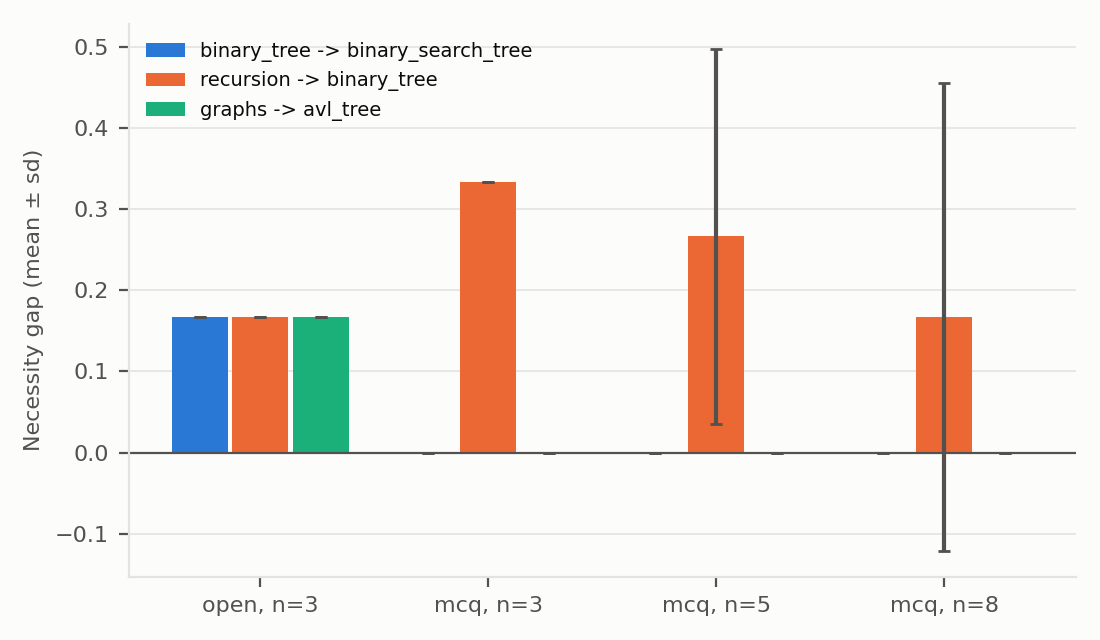
\includegraphics[width=\columnwidth]{necessity_gap_stability.png}
\caption{Necessity gap by setting and edge; error bars show SD across three seeds. No setting shows the expected order.}
\end{figure}
A plausible explanation is that a small LLM cannot reliably simulate not knowing a concept, since it answers partly from its own knowledge. This is a hypothesis and we have not tested it directly. We keep the test as report-only, and RQ1 includes a setting that gives it weight, to measure its effect on real data.

\subsection{RQ2 and RQ4: Simulated Students}
Table VI uses 500 simulated students per condition on a five-concept example graph, target AVL tree. When knowledge follows the graph, adaptive diagnosis saved 14.4\% of questions at nearly the same accuracy as asking everything, and beat random order at the same budget. When knowledge ignores the graph, adaptive saved 27.2\% of questions but lost about 10 accuracy points, so its advantage depends on the graph being a good model of the student.

\begin{table}[!t]
\caption{Diagnosis on Simulated Students (RQ2)}
\centering\footnotesize
\begin{tabular}{@{}p{0.386\columnwidth}p{0.313\columnwidth}p{0.221\columnwidth}@{}}
\toprule
\textbf{Students / strategy} & \textbf{Avg. questions} & \textbf{Accuracy} \\ \midrule
\textbf{Follow the graph} &  &  \\
Adaptive & 4.28 & 0.866 \\
Ask every concept & 5.00 & 0.870 \\
Random, same budget & 4.28 & 0.824 \\
\textbf{Ignore the graph} &  &  \\
Adaptive & 3.64 & 0.775 \\
Ask every concept & 5.00 & 0.874 \\
Random, same budget & 3.64 & 0.759 \\
\bottomrule
\end{tabular}
\end{table}
Table VII shows that personalized paths are much shorter than the generic path of five concepts, but they do not cover every gap, because diagnosis makes errors. The shorter path in the second condition comes with far lower coverage (0.59). Order violations are 0 in both conditions, but that follows from topological sorting of the same graph, so it says little by itself.

\begin{table}[!t]
\caption{Personalized vs. Generic Paths (RQ4)}
\centering\footnotesize
\begin{tabular}{@{}p{0.368\columnwidth}p{0.276\columnwidth}p{0.276\columnwidth}@{}}
\toprule
\textbf{Measure} & \textbf{Follow graph} & \textbf{Ignore graph} \\ \midrule
Generic path length & 5.00 & 5.00 \\
Personalized length & 2.35 & 1.77 \\
Length reduction & 52.9\% & 64.6\% \\
Gap coverage & 0.81 & 0.59 \\
Order violations & 0 & 0 \\
\bottomrule
\end{tabular}
\end{table}
\subsection{RQ3: Root-Cause Tracing (Dev Set Only)}
On a 10-item development set with no mastery information, the LLM tracer tied the blame-the-target baseline (top-1 0.5, top-3 0.8), and blame-the-nearest reached top-1 0.4, top-3 0.8. Ten items cannot separate these methods. The tracer is now frozen, and it will be evaluated once on the 40-item test set, which shares no quiz items with the development set.

\subsection{Inter-Annotator Agreement (Pilot)}
On 20 pairs labelled by two authors, raw $\kappa$ was 0.49 (ds101 0.85, ml101 0.17). After the shortcut rule it was 0.77 (ds101 1.00, ml101 0.55). The rule changed four labels of one annotator and none of the other's, because the second annotator's labels had already had the rule applied during labelling, so raw $\kappa$ partly reflects that difference. Seven pairs are ties awaiting adjudication. These pairs are a pilot chosen before the real concept list existed.

\subsection{RQ1: Edge Quality}
Precision, recall and F1 for all settings are pending. The scoring harness, baselines, ablation flags and benchmark sampler are implemented, but we report no RQ1 numbers until the runs are complete.

\section{Limitations}
\begin{itemize}
\item \textbf{Most results are preliminary.} RQ1 and RQ3 have no test results yet. RQ2 and RQ4 use a five-concept example graph, not a real course.
\item \textbf{Simulated students share the graph they evaluate.} The first condition assumes knowledge follows the graph, so it shows performance given a correct graph, not that real students behave this way.
\item \textbf{Small pilot gold.} Twenty pairs by two student annotators cannot support strong conclusions, and agreement on ml101 was low.
\item \textbf{Benchmarks test only part of the agent.} With no course text, the evidence and necessity checks do not run there. Only two benchmarks are used, from the same group.
\item \textbf{Uncalibrated thresholds, and one prompt change on pilot edges.} Decision values are a first choice. Semantic prompt v2 was changed once after we saw example edges that overlap the pilot gold, so those pairs must be excluded from final scores.
\item \textbf{Discovery is not yet good enough.} Concept filtering is too permissive, and prompt v3 is not yet proven at scale. The fixed concept order in v3 may itself bias answers, and we will check its effect before reporting results.
\item \textbf{Hardware.} Two models do not fit together in 8 GB of memory, which limited how much we could run. Out-of-memory errors can silently affect results, so such runs are discarded.
\end{itemize}
\section{Future Work}
The immediate work is to complete the evaluation: run RQ1 on the benchmarks and full courses, tighten concept filtering, label a larger gold set of real concepts, calibrate and freeze thresholds, then run RQ3 once and repeat RQ2 and RQ4 on real graphs. A small pre/post study with real students is planned. Later directions include better ways to test necessity, cross-course graphs, and learning thresholds from teacher decisions.

\section{Conclusion}
We built an end-to-end system in which LLM-proposed prerequisites are treated as claims to check. Validated edges then support an adaptive quiz and a personal learning path. Our early findings are mixed and useful. Simulating a learner's missing knowledge was unstable, a real textbook exposed silent failures in discovery, and adaptive diagnosis saves questions mainly when knowledge follows the graph. Whether the agent improves edge quality remains to be measured, and that is the next step.

\section*{Acknowledgment}
The authors thank the Department of Computer Science \& Engineering, M S Ramaiah Institute of Technology. Parts of the software and of this manuscript's text were drafted with an AI coding assistant (Anthropic's Claude, through Claude Code), including the mechanical application of the shortcut rule to one annotator's answers. The authors directed this work and remain responsible for it. The LLMs used inside the method are described in Section IV.
\begin{thebibliography}{99}
\bibitem{pan_kg} S. Pan, L. Luo, Y. Wang, C. Chen, J. Wang, and X. Wu, ``Unifying large language models and knowledge graphs: A roadmap,'' \emph{IEEE Trans. Knowl. Data Eng.}, vol. 36, no. 7, pp. 3580--3599, 2024.
\bibitem{ji_halluc} Z. Ji et al., ``Survey of hallucination in natural language generation,'' \emph{ACM Comput. Surv.}, vol. 55, no. 12, pp. 1--38, 2023.
\bibitem{talukdar} P. P. Talukdar and W. W. Cohen, ``Crowdsourced comprehension: Predicting prerequisite structure in Wikipedia,'' in \emph{Proc. 7th Workshop Building Educ. Appl. Using NLP}, 2012, pp. 307--315.
\bibitem{refd} C. Liang, Z. Wu, W. Huang, and C. L. Giles, ``Measuring prerequisite relations among concepts,'' in \emph{Proc. EMNLP}, 2015, pp. 1668--1674.
\bibitem{pan_mooc} L. Pan, C. Li, J. Li, and J. Tang, ``Prerequisite relation learning for concepts in MOOCs,'' in \emph{Proc. ACL}, 2017, pp. 1447--1456.
\bibitem{liang17} C. Liang, J. Ye, Z. Wu, B. Pursel, and C. L. Giles, ``Recovering concept prerequisite relations from university course dependencies,'' in \emph{Proc. AAAI}, 2017, pp. 4786--4791.
\bibitem{liang18} C. Liang, J. Ye, S. Wang, B. Pursel, and C. L. Giles, ``Investigating active learning for concept prerequisite learning,'' in \emph{Proc. AAAI (EAAI)}, 2018, pp. 7913--7919.
\bibitem{prereq} S. Roy, M. Madhyastha, S. Lawrence, and V. Rajan, ``Inferring concept prerequisite relations from online educational resources,'' in \emph{Proc. AAAI}, vol. 33, 2019, pp. 9589--9594.
\bibitem{lecturebank} I. Li, A. R. Fabbri, R. R. Tung, and D. R. Radev, ``What should I learn first: Introducing LectureBank for NLP education and prerequisite chain learning,'' in \emph{Proc. AAAI}, vol. 33, 2019, pp. 6674--6681.
\bibitem{pcpl} F. Du, W. Hu, C. Qin, and Z. Xiao, ``A prompt-based approach for discovering prerequisite relations among concepts,'' in \emph{Proc. ITEI 2023}, Zhengzhou, China, EAI, 2024, doi: 10.4108/eai.24-11-2023.2343577.
\bibitem{lcpre} J. Sun, Y. He, Y. Xu, J. Sun, and G. Sun, ``A learning-path based supervised method for concept prerequisite relations extraction in educational data,'' in \emph{Proc. CIKM}, 2024, pp. 2168--2177.
\bibitem{gkrom} M. Zhang, J. Wang, K. Xiao, S. Wang, Y. Zhang, H. Chen, and Z. Li, ``Learning concept prerequisite relation via global knowledge relation optimization,'' in \emph{Proc. AAAI}, vol. 39, no. 2, 2025, pp. 1638--1646.
\bibitem{ace} M. C. Aytekin and Y. Sayg{\i}n, ``ACE: AI-assisted construction of educational knowledge graphs with prerequisite relations,'' \emph{J. Educ. Data Mining}, vol. 16, no. 2, pp. 85--114, 2024.
\bibitem{instructkg} A. AlRabah, P. Kargupta, J. Han, and A. Alawini, ``Instructor-aligned knowledge graphs for personalized learning,'' arXiv:2602.17111, 2026.
\bibitem{chanaa} A. Chanaa and N. El Faddouli, ``Prerequisites-based course recommendation: Recommending learning objects using concept prerequisites and metadata matching,'' \emph{Smart Learn. Environ.}, vol. 11, art. 16, 2024.
\bibitem{kst} J.-P. Doignon and J.-C. Falmagne, ``Spaces for the assessment of knowledge,'' \emph{Int. J. Man-Machine Studies}, vol. 23, no. 2, pp. 175--196, 1985.
\bibitem{bkt} A. T. Corbett and J. R. Anderson, ``Knowledge tracing: Modeling the acquisition of procedural knowledge,'' \emph{User Model. User-Adapt. Interact.}, vol. 4, no. 4, pp. 253--278, 1994.
\bibitem{dkt} C. Piech et al., ``Deep knowledge tracing,'' in \emph{Adv. Neural Inf. Process. Syst.}, vol. 28, 2015.
\bibitem{rag} P. Lewis et al., ``Retrieval-augmented generation for knowledge-intensive NLP tasks,'' in \emph{Adv. Neural Inf. Process. Syst.}, vol. 33, 2020, pp. 9459--9474.
\bibitem{selfcons} X. Wang et al., ``Self-consistency improves chain of thought reasoning in language models,'' in \emph{Proc. ICLR}, 2023.
\bibitem{judge} L. Zheng et al., ``Judging LLM-as-a-judge with MT-Bench and Chatbot Arena,'' in \emph{Adv. Neural Inf. Process. Syst. Datasets and Benchmarks Track}, 2023.
\bibitem{sbert} N. Reimers and I. Gurevych, ``Sentence-BERT: Sentence embeddings using Siamese BERT-networks,'' in \emph{Proc. EMNLP-IJCNLP}, 2019, pp. 3982--3992.
\bibitem{ods} P. Morin, \emph{Open Data Structures (in pseudocode)}, Edition 0.1G$\beta$. [Online]. Available: \url{https://opendatastructures.org/}
\bibitem{opendsa} OpenDSA Project, OpenDSA modules, GitHub repository, commit f900a7a.
\bibitem{d2l} A. Zhang, Z. C. Lipton, M. Li, and A. J. Smola, \emph{Dive into Deep Learning}, release 1.0.3. [Online]. Available: \url{https://d2l.ai/}
\bibitem{ims} M. \c{C}etinkaya-Rundel and J. Hardin, \emph{Introduction to Modern Statistics}, 2nd ed., OpenIntro.
\bibitem{cohen} J. Cohen, ``A coefficient of agreement for nominal scales,'' \emph{Educ. Psychol. Meas.}, vol. 20, no. 1, pp. 37--46, 1960.
\end{thebibliography}
\end{document}